\documentclass{standalone}

\usepackage{tikz}
\usetikzlibrary{calc,snakes}

\begin{document}

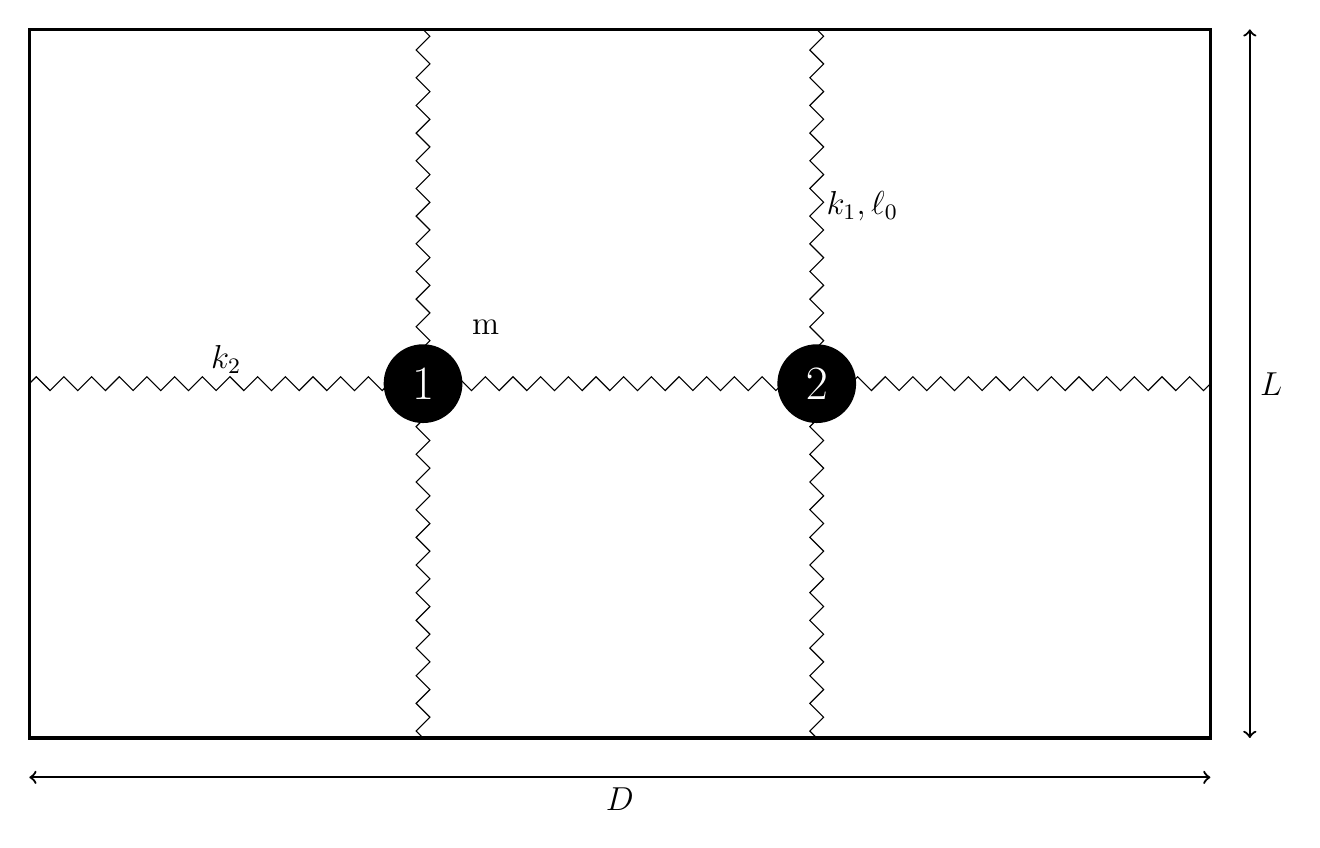
\begin{tikzpicture}

\coordinate (A) at (5  , 4.5);
\coordinate (B) at (10 , 4.5);

\draw[very thick](0,0)rectangle(15,9);

\draw[thick,<->] (15.5,0)--node[anchor=west]{\large $L$}(15.5,9);
\draw[thick,<->] (0,-0.5)--node[anchor=north]{\large $D$}(15,-0.5);

\draw[snake=zigzag](5  , 0)   -- (A);
\draw[snake=zigzag](5  , 9)   -- (A);
\draw[snake=zigzag](10 , 0)   -- (B);
\draw[snake=zigzag](10 , 9)   -- node[anchor=west]{\large $k_1, \ell_0$}(B);
\draw[snake=zigzag](0  , 4.5) -- node[anchor=south]{\large $k_2$}(A);
\draw[snake=zigzag](15 , 4.5) -- (B);
\draw[snake=zigzag](A)        -- (B);

\fill(A)node{\color{white}\LARGE 1} circle (0.5); 
\node[anchor=south west] at ($(A)+(0.5,0.5)$){\large m};
\fill(B)node{\color{white}\LARGE 2}circle (0.5);

\end{tikzpicture}

\end{document}
